\chapter{Functional Tests}\label{C:Functional-Tests}
Simultaneously with the development of IOSharp some small tests were created so the developed features could be tested to verify the properly operation of the implementation. Two functional test had been carried out in order to test the correct functioning of the library. The first one uses a Micro Framework project which consists of a RFID card reader. The second one is mainly the deployment of HomeSense.

\section{SPI. RFID and IOSharp}\label{S:rfid-iosharp}
This was the first test to verify the SPI in a real environment using a RFID card reader connected through the SPI bus. This test derives from a proof of concept made for VR gym in Argentona under the Spanish project "Activat" from "Proyecto Impacto". This project requested to develop a method to authenticate and authorize users for a secure entrance on a complex by using a RFID card reader and different cards, tags and wristbands with an ID which can be associated with a certain user.
\\
The project was developed using a Netduino Plus which uses Micro Framework. The card reader used in this test mounts a MFRC522 chip from NXP which can use different communication protocols like SPI, UART and \gls{I2C}. But that chip is mounted on a MF522-AN board from Mifare which only offers a SPI interface.
\\
An API was written in order to communicate the Netduino with the card reader, so the MFRC522 datasheet was used (see on Appendix \ref{C:Libraries-Datasheets} the section \ref{SS:Libs-MFRC522-Datasheet}). The program creates an instance of this API and then starts the SPI configuration. Following this configuration a Timer is instantiated which triggers a function at the scheduled cycle. The called function uses the API to communicate with the card reader so it can retrieve the card ID and then, with another tranmission, obtain the Serial Number located in the card. Finally it prints this data in the console.

\subsection{Micro Framework version}\label{S:IOEx-SPI-Netduino}
The original example uses Micro Framework and the Secretlab classes for the Netduino Plus so the resulting binary will only work on this board. The port configuration for this example is really simple, because it only uses a pin for the \gls{CS}. The \gls{MOSI}, \gls{MISO} and \gls{SCLK} are defined by the board schema so the pins will be selected and configured internally on the virtual machine.

\begin{lstlisting}[language=CSharp, caption={SPIApi.cs - Configuring SPI for the MFRC522 in Netduino Plus}]
public void ConfigureSPI() {
    SPI.Configuration xSPIConfig;
    Cpu.Pin pin = Pins.GPIO_PIN_D9;

    xSPIConfig = new SPI.Configuration(pin, //Chip Select pin
        false, //Chip Select Active State
        50, //Chip Select Setup Time
        0, //Chip Select Hold Time
        false, //Clock Idle State
        true, //Clock Edge
        1000, //Clock Rate (kHz)
        SPI.SPI_module.SPI1); //SPI Module
    spiDevice = new SPI(xSPIConfig);
}
\end{lstlisting}
As it is shown above, the \gls{CS} pin is the \verb!Pins.GPIO_PIN_D9! which corresponds to a digital pin.

\subsection{Migrating to Linux}\label{S:IOEx-SPI-Migrating-to-IOSharp}
To use IOSharp instead of Micro Framework there is not a big requirement, basically the project must be converted to .NET Framework and then reference the IOSharp library. Beside this, the mapping classes according to the deployment platform must also be referenced. The next step is change the pin for the \gls{CS} to the according one. Normally in Linux each SPI device have one or more \gls{CS} pins but not every pin is suitable to work with that SPI device, so it is important to check the appropriate pin.
\\
Taking in mind that using this test can also prove that IOSharp can work with the original code by doing a minimal set of changes, it was tried to use one of the features that the Visual Studio projects offers. Declaring two solution files (\verb!*.sln!) which each one calls two different project files (\verb!*.csproj!) make possible to have one solution with the Micro Framework classes for the Netduino while the other one contains the references for the IOSharp and the .NET Framework. This will create two different projects from the same code, one being able to run on Netduino and the other one in Linux.
\\
These were the major changes, and they cannot be considered real changes to the original code, because is possible to take the application program and create a new .NET Framework project with that code. This changes proves that is possible to maintain the same code for different platform deployments.
\\
Using conditional compiling is possible to set the required pin for each board and each solution. In this case, the symbol used for the conditional compiling is \verb!MF! which is present on the Netduino version of the \verb!*.csproj! whereas not in the Raspberry Pi. Taking a look into the above code, the Netduino uses \verb!Pins.GPIO_PIN_D9! whereas the Raspberry Pi uses \verb!Cpu.Pin.GPIO_Pin9!.

\begin{lstlisting}[language=CSharp, caption={SPIApi.cs - Conditional compiling symbol for NETMF and IOSharp}]
public void ConfigureSPI() {
    SPI.Configuration xSPIConfig;
    Cpu.Pin pin = Cpu.Pin.GPIO_NONE;
  	// In this case, the conditional compiling symbol used is MF, true for Micro Framework or false for IOSharp
  	#if MF
    	pin = Pins.GPIO_PIN_D9;
    #else
        pin = Cpu.Pin.GPIO_Pin9;
    #endif

    xSPIConfig = new SPI.Configuration(pin, //Chip Select pin
        false, //Chip Select Active State
        50, //Chip Select Setup Time
        0, //Chip Select Hold Time
        false, //Clock Idle State
        true, //Clock Edge
        1000, //Clock Rate (kHz)
        SPI.SPI_module.SPI1); //SPI Module
    spiDevice = new SPI(xSPIConfig);
    //MFRC522Init();
}
\end{lstlisting}

After doing this, this project can be opened as Micro Framework in order to deploy in a Netduino or open the Linux version. Deploying this application in any of these boards will result in a working program like the figure \ref{fig:IOEx-SPI} shows.
\begin{figure}[H]\begin{center}
 \centering
  \captionsetup{justification=centering}
  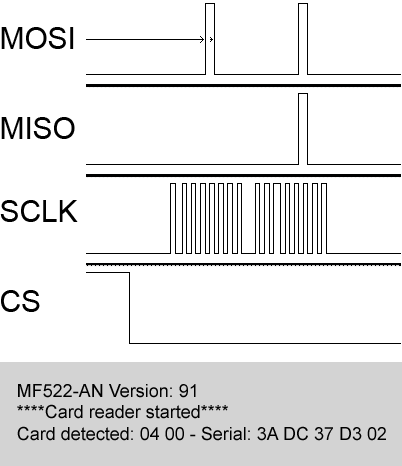
\includegraphics[width=0.5\textwidth]{pictures/examples/rfid-spi}
  \caption{Data exchange using the SPI\label{fig:IOEx-SPI}}
\end{center}\end{figure}

\section{HomeSense}\label{S:IOEx-HomeSense}
HomeSense is a Wireless Healthcare Sensor Platform designed by AlterAid. The current implementation uses a Netduino Mini board which is the gateway. This board controls the sensor network, receiving all the data and uploading it to internet. Some sensors are spread around the house which are used to fetch data. With all of those sensors, it is possible to acquire information from the environment and then send that information to internet using the gateway.
\\
These sensors are programmed using C and all of them use the \gls{SoC} nRF24LE1 which mounts a low-power RF ISM band (2.4 GHz) from Nordic Semiconductor.
\begin{figure}[H]\begin{center}
 \centering
  \captionsetup{justification=centering}
  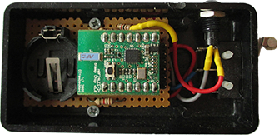
\includegraphics[scale=1]{pictures/examples/sensor}
  \caption{Sensor for a medicine cabinet\label{fig:IOEx-UART}}
\end{center}\end{figure}
The communication protocol designed for HomeSense is similar to a star network with multi-hop transmissions so it becomes a tree-start topology. The nodes try to fetch the gateway because this is on charge of upload the information to the internet.

\subsection{Gateway}\label{SS:IOEx-HomeSense-Gateway}
The program running on the gateway is coded using Micro Framework and is deployed on a Netduino Mini. Using IOSharp has been possible to deploy it on a Raspberry Pi running Linux and Mono. The software running on the gateway controls the communication hardware and also the mesh network using the designed protocol for this platform.
\\
As it uses all the features developed for the library it is a good functional test to try the whole system.

\begin{itemize}
\item \textbf{UART}: the Serial Port is used to transmit data between the Wifly and the Raspberry Pi. The Wifly is an XBee socket type module created by Roving Networks, and is used to connect to Wi-Fi networks. The communication between this module and the board where is connected is carried out using UART with a protocol described on the specification paper provided by the manufacturers.

\item \textbf{SPI}: The Nordic nRF24L01+ is controlled using the SPI protocol. This chip is used to create the physical meshed network which connects with the different nodes. The channel created using the Nordic is half-duplex so there is only one communication at a time either transmission or reception.
\item \textbf{Interrupts}: When the gateway's Nordic receives information form other nodes it must alert that new data is waiting to be read, to make this alert an interruption is used on a GPIO
\end{itemize}
Figure \ref{fig:IOEx-GW-Diagram} summarizes the connections and devices used with the Raspberry Pi and HomeSense. On the left is shown the Nordic which uses the SPI protocol and it send interrupts to the Raspberry Pi. On the right, the Wifly uses the UART protocol to exchange data.
\begin{figure}[H]\begin{center}
 \centering
  \captionsetup{justification=centering}
  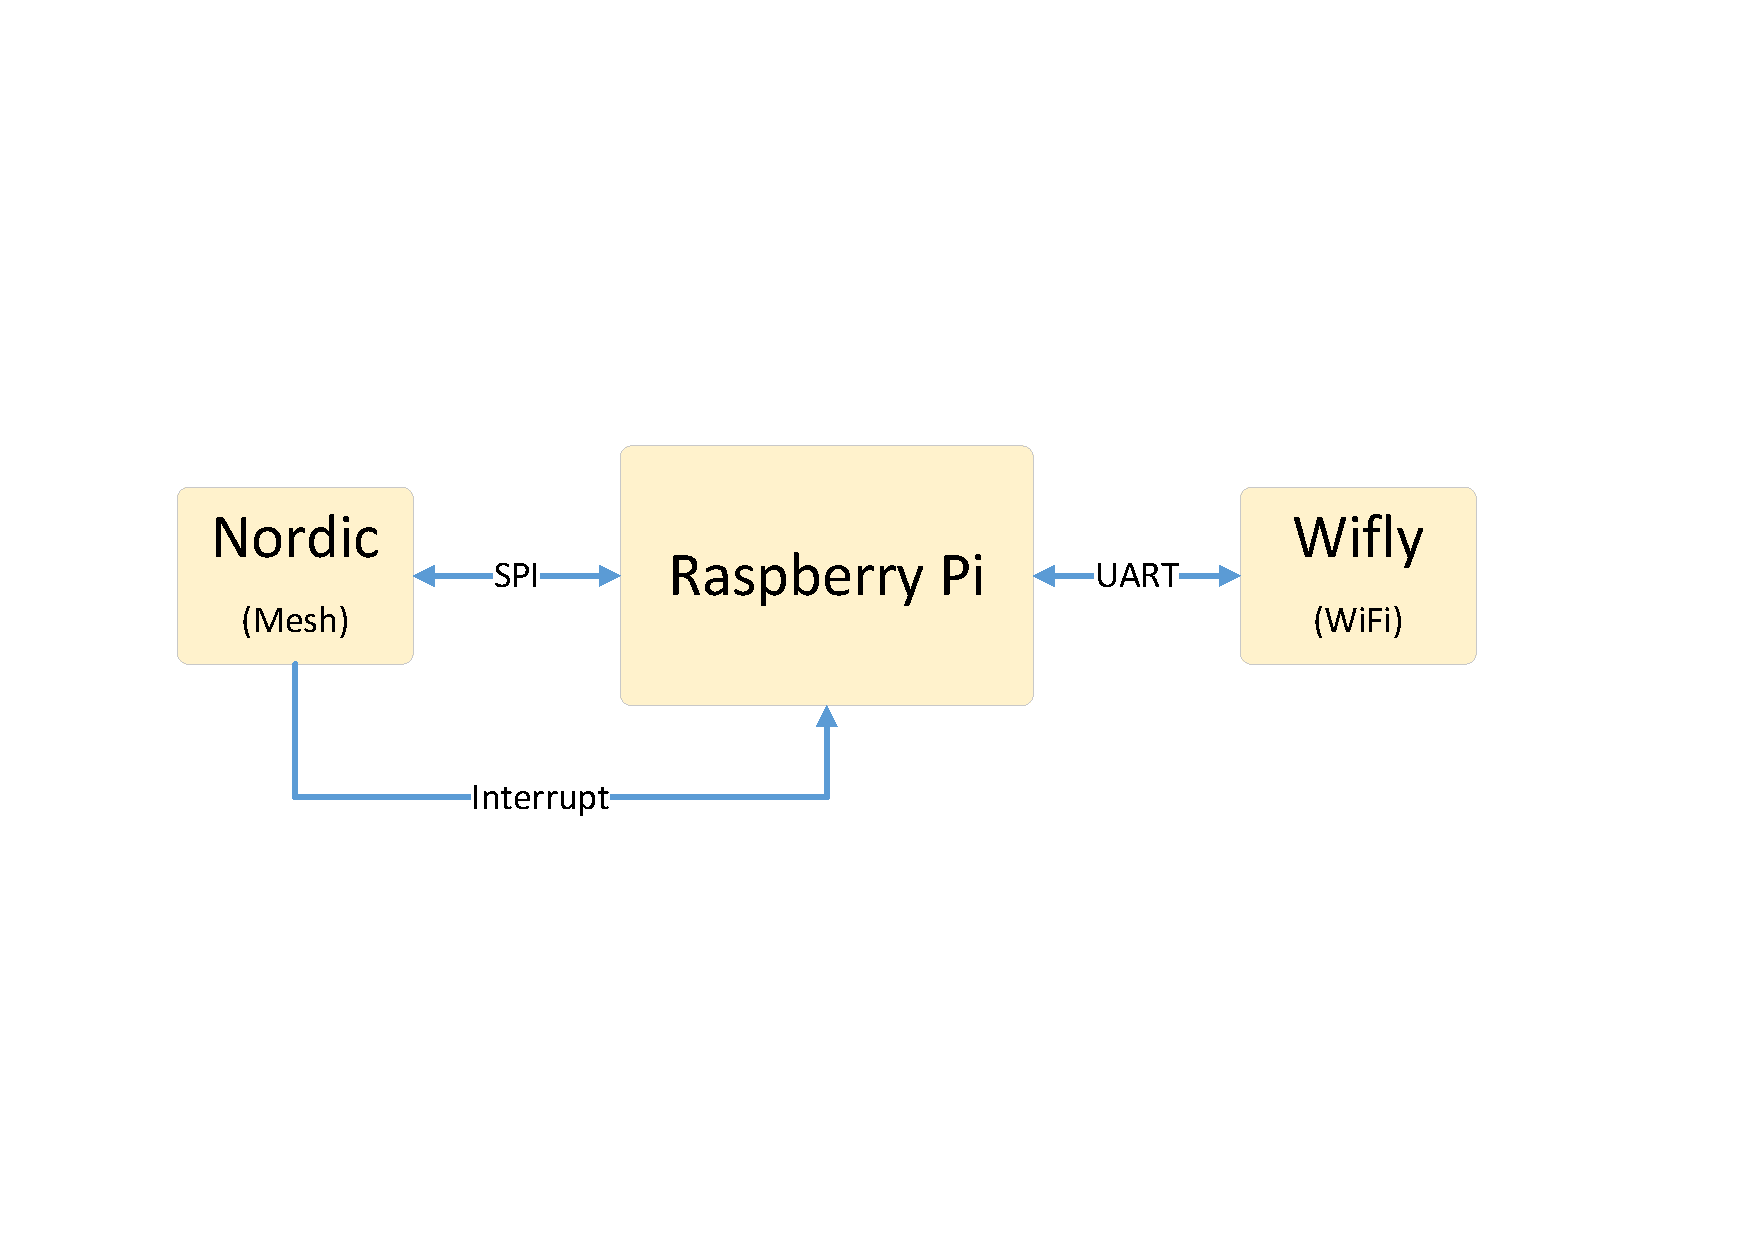
\includegraphics[width=0.8\textwidth]{pictures/examples/gateway-diagram}
  \caption{Diagram showing the protocols and devices used in HomeSense\label{fig:IOEx-GW-Diagram}}
\end{center}\end{figure}
With all of these devices attached to the shield used in the Raspberry Pi it will be possible to test all the functions working at the same time and how the system response is compared to the original one.
\begin{figure}[H]\begin{center}
 \centering
  \captionsetup{justification=centering}
  \includegraphics[width=0.6\textwidth]{pictures/examples/raspihomestack}
  \caption{Raspberry Pi with the modules needed to run HomeSense\label{fig:IOEx-HS-Stack}}
\end{center}\end{figure}

\subsection{Working}\label{SS:IOEx-HomeSense-Working}
As IOSharp has implemented all the features required in HomeSense, it is possible to change the project type from Micro Framework to .NET Framework and then reference this library. Finally, the ports need to be remapped according to the shield used with the Raspberry Pi. The strategy to do this mapping is include the Hardware class of the Raspberry Pi and then rename the ports to the according ones. SerialPort device also must be renamed from \verb!COM1! to \verb!/dev/ttyAMA0!. After changing the references and the port names is possible to start testing the program. So it has been really easy to migrate from the Netduino Mini board to the Raspberry Pi.
\\
\\
HomeSense has a program which shows the network status, showing its gateway and the different sensors connected to the network. On the following figure a connection is shown. The aaaida logo represents the gateway whereas the node is represented by a door. In this case, both are linked as an arrow connects both of them. With this program is possible to know the network addresses of both devices. Also it shows other information like battery state or the fetched information by any sensor located on a node.
\begin{figure}[H]\begin{center}
 \centering
  \captionsetup{justification=centering}
  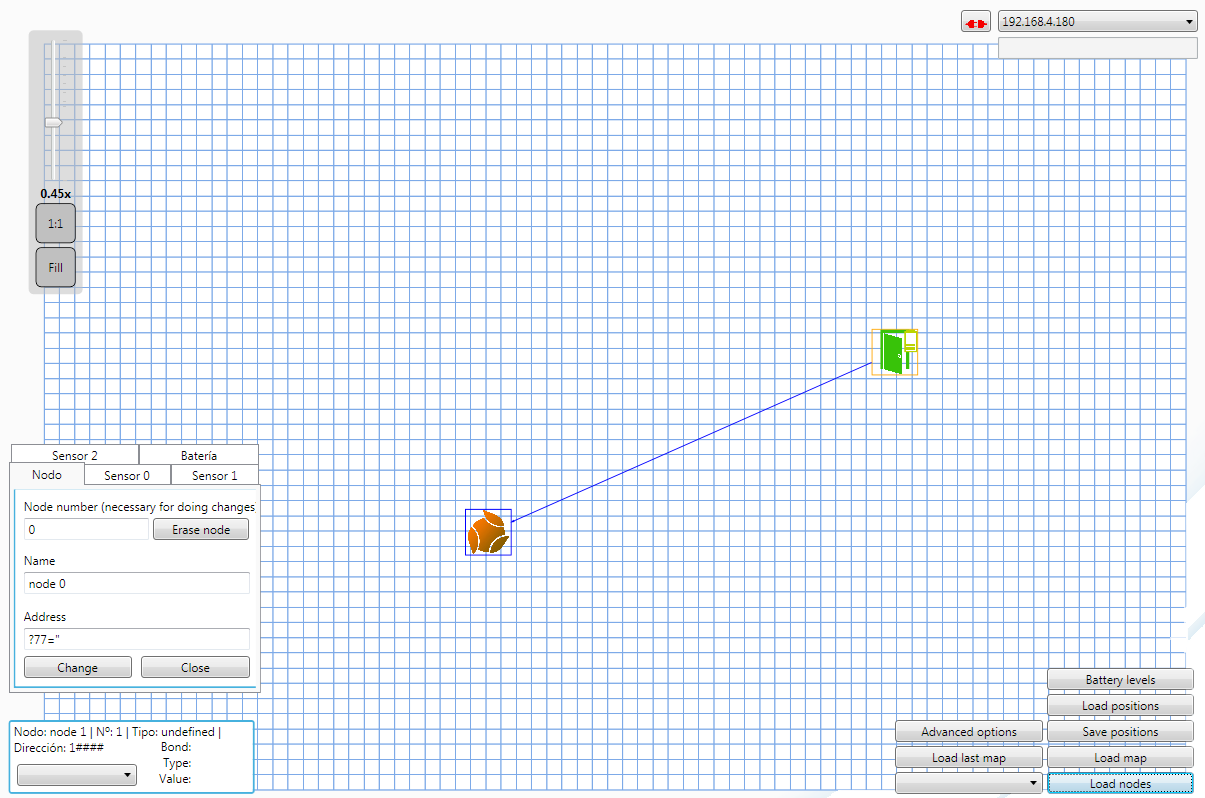
\includegraphics[width=1\textwidth]{pictures/examples/homesense-pillin}
  \caption{HomeSense dashboard. The aaaida logo on the left represents the Raspberry Pi (gateway)  whereas the door represents a sensor\label{fig:IOEx-HS-Dash}}
\end{center}\end{figure}

\section{Conclusions}\label{S:Results-overview}
All the functional tests show that IOSharp has been successfully done. Each test works on the Raspberry Pi with doing only minor changes on the code. With IOSharp working and being able to be used on existing Micro Framework projects it is possible to make them run on other platforms, so the development milestone has been done. But, after testing the different parts of IOSharp and deploying HomeSense on the Raspberry Pi it was seen that the performance was not as good as it was expected. Raspberry Pi, need more time to send the network events than the Netduino and this is probably related to the time needed to attend the interrupts on Mono. In this case the IOSharp with Mono needs two transmissions to send the same information that is sent with only one transmission in the Netduino.
\\
To try to solve these issues with the performance of the library, IOSharp will be translated to C++ using a translating tool called AlterNative which is capable of translate .NET assemblies to C++ while maintaining a similar C\# syntax.